%%%%%%%%%%%%%%%%%%%%%%%%%%%%%%%%%%%%%%%%%%%%%%%%%%%%%%%%%%%%%%%%%%%%%%%%%%%%%%%%%%%%%%%%%%%%%%%%
%
% CS484 Written Question Template
%
% Acknowledgements:
% The original code is written by Prof. James Tompkin (james_tompkin@brown.edu).
% The second version is revised by Prof. Min H. Kim (minhkim@kaist.ac.kr).
%
% This is a LaTeX document. LaTeX is a markup language for producing 
% documents. Your task is to fill out this document, then to compile 
% it into a PDF document. 
%
% 
% TO COMPILE:
% > pdflatex thisfile.tex
%
% If you do not have LaTeX and need a LaTeX distribution:
% - Personal laptops (all common OS): www.latex-project.org/get/
% - We recommend latex compiler miktex (https://miktex.org/) for windows,
%   macTex (http://www.tug.org/mactex/) for macOS users.
%   And TeXstudio(http://www.texstudio.org/) for latex editor.
%   You should install both compiler and editor for editing latex.
%   The another option is Overleaf (https://www.overleaf.com/) which is 
%   an online latex editor.
%
% If you need help with LaTeX, please come to office hours. 
% Or, there is plenty of help online:
% https://en.wikibooks.org/wiki/LaTeX
%
% Good luck!
% Min and the CS484 staff
%
%%%%%%%%%%%%%%%%%%%%%%%%%%%%%%%%%%%%%%%%%%%%%%%%%%%%%%%%%%%%%%%%%%%%%%%%%%%%%%%%%%%%%%%%%%%%%%%%
%
% How to include two graphics on the same line:
% 
% \includegraphics[\width=0.49\linewidth]{yourgraphic1.png}
% \includegraphics[\width=0.49\linewidth]{yourgraphic2.png}
%
% How to include equations:
%
% \begin{equation}
% y = mx+c
% \end{equation}
% 
%%%%%%%%%%%%%%%%%%%%%%%%%%%%%%%%%%%%%%%%%%%%%%%%%%%%%%%%%%%%%%%%%%%%%%%%%%%%%%%%%%%%%%%%%%%%%%%%

\documentclass[11pt]{article}

\usepackage[english]{babel}
\usepackage[utf8]{inputenc}
\usepackage[colorlinks = true,
            linkcolor = blue,
            urlcolor  = blue]{hyperref}
\usepackage[a4paper,margin=1.5in]{geometry}
\usepackage{stackengine,graphicx}
\usepackage{fancyhdr}
\setlength{\headheight}{15pt}
\usepackage{microtype}
\usepackage{times}
\usepackage{booktabs}
\usepackage{graphicx}
\usepackage{amsmath}

% From https://ctan.org/pkg/matlab-prettifier
\usepackage[numbered,framed]{matlab-prettifier}

\frenchspacing
\setlength{\parindent}{0cm} % Default is 15pt.
\setlength{\parskip}{0.3cm plus1mm minus1mm}

\pagestyle{fancy}
\fancyhf{}
\lhead{Homework Writeup}
\rhead{CS484}
\rfoot{\thepage}

\date{}

\title{\vspace{-1cm}Homework 4 Writeup}


\begin{document}
\maketitle
\vspace{-3cm}
\thispagestyle{fancy}

\section*{Instructions}
\begin{itemize}
  \item Describe any interesting decisions you made to write your algorithm.
  \item Show and discuss the results of your algorithm.
  \item Feel free to include code snippets, images, and equations.
  \item Use as many pages as you need, but err on the short side If you feel you only need to write a short amount to meet the brief, th
  
  \item \textbf{Please make this document anonymous.}
\end{itemize}

\newcommand\tab[1][1cm]{\hspace*{#1}}
\section*{Files\&Algorithm}  

{\large $1.$ bayer\_to\_rgb\_bicubic.m \par}
\tab input : bayer\_img (RGBG) \\
\tab output : rgb\_img (RGB)

\tab I used bilinear interpolation to change bayer image to rgb image. \\
\tab $1)$ Make zero image. \\
\tab $2)$ Get size of bayer image. \\
\tab $3)$ There are two case of Green. First, $mod(i,2) == 0 \&\& mod(j,2)== 1.$ \\ \tab \ \ Second is  $mod(i,2) == 1 \&\& mod(j,2) == 0.$\\
\tab $4)$ Case of Red is mod(i,2) == 1. Else is case of Blue \\

{\large $2.$ calculate\_fundamental\_matrix.m \par}
\tab input : pts$1$, pts$2$ (feature point) \\
\tab output : f (Fundamental matrix)

\tab $1)$ Make array A. \\
\tab $2)$ Using svd function, get smallest eigenvector of $A^TA$ . \\
\tab $3)$ $F=reshape(eigenvector)$.\\
\tab $4)$ $F=USV^T$ \\
\tab $5)$ Make minimum singular value for S become zero. \\
\tab $6)$ $F=USV^T$ by using modified S at $5)$ \\

\newpage
{\large $3.$ calculate\_rectification\_matrix.m \par}
\tab input : f (Fundamental matrix), imageSize, pts$1$, pts$2$ \\
\tab output : t$1$, t$2$ \\

\tab $1)$ Make u,d,v of f with svd function. \\
\tab $2)$ Make $epipole = u_3$ \\
\tab $3)$ $t = [1\ 0\ -w./2;\ 0\ 1\ -h./2;\ 0\ 0\ 1]$ \\
\tab $4)$ $theta = atan(p2t(2)/p2t(1));$ \\
\tab $5)$ $r = [cos(-theta)\ -sin(-theta)\ 0;\ sin(-theta)\ cos(-theta)\ 0;\ 0\ 0\ 1]$ \\
\tab $6)$ $g = [1\ 0\ 0;\ 0\ 1\ 0;\ -1/ex\ 0\ 1]$ \\

{\large $4.$ calculat\_disparity\_map.m \par}
\tab Make a cost volume using NCC(normalized cross correlation) matching cost function for the two rectified images, then obtain disparity map from the cost volume after aggregate it with a box filter. \\\\


\section*{In code.}
{\large $1.$ bayer\_to\_rgb\_bicubic.m \par}
\begin{lstlisting}[style=Matlab-editor]
function rgb_img = bayer_to_rgb_bicubic(bayer_img)
    [M,N,L] = size(bayer_img);
    img = uint8(zeros(M,N,3));
    for i = 2:M-1
        for j = 2:N-1
            if mod(i,2) == 0 && mod(j,2) == 1 \%G
                img(i,j,1)=round((bayer_img(i-1,j)+bayer_img(i+1,j))/2);
                img(i,j,2)=round(bayer_img(i,j));
                img(i,j,3)=round((bayer_img(i,j-1)+bayer_img(i,j+1))/2);
            elseif mod(i,2) == 1 && mod(j,2) == 0
                img(i,j,1)=round((bayer_img(i,j-1)+bayer_img(i,j+1))/2);
                img(i,j,2)=round(bayer_img(i,j));
                img(i,j,3)=round((bayer_img(i-1,j)+bayer_img(i+1,j))/2);
            elseif mod(i,2) == 1 \%R
                img(i,j,1)=round(bayer_img(i,j));
                img(i,j,2)=round((bayer_img(i-1,j)+bayer_img(i+1,j)+bayer_img(i,j-1)+bayer_img(i,j+1))/4);
                img(i,j,3)=round((bayer_img(i-1,j-1)+bayer_img(i+1,j-1)+bayer_img(i+1,j-1)+bayer_img(i-1,j+1))/4);
            else \%B
                img(i,j,1)=round((bayer_img(i-1,j-1)+bayer_img(i+1,j-1)+bayer_img(i+1,j-1)+bayer_img(i-1,j+1))/4);
                img(i,j,2)=round((bayer_img(i-1,j)+bayer_img(i+1,j)+bayer_img(i,j-1)+bayer_img(i,j+1))/4);
                img(i,j,3)=round(bayer_img(i,j));
            end
        end
    end
    bayer_img = img;
    rgb_img = bayer_img;
\end{lstlisting}


{\large $2.$ calculate\_fundamental\_matrix.m \par}
\begin{lstlisting}[style=Matlab-editor]
function f = calculate_fundamental_matrix(pts1, pts2)
    [m,~] = size(pts1);
    X1 = pts1(:, 1);    Y1 = pts1(:, 2);
    X2 = pts2(:, 1);    Y2 = pts2(:, 2);
    A = [X1.*X2, X1.*Y2, X1, Y1.*X2, Y1.*Y2, Y1, X2, Y2, ones(m,1)];

    [~,~,EV1] = svd(A);

    EV = EV1(:,9);

    F = reshape(EV,3,3);

    [U,S,V] = svd(F);
    S(3,3) = 0;
    F = U*S*V';
    f = F;
\end{lstlisting}
\[
A=
  \begin{bmatrix}
    $xx'$ & $xy'$ & $x$ & $yx'$ & $yy'$ & $y$ & $x'$ & $y'$ & 1 \\
    $... $ & $...$ & $...$ & $...$ & $...$ & $...$ & $...$ & $...$ & $...$ \\
    $xx'$ & $xy'$ & $x$ & $yx'$ & $yy'$ & $y$ & $x'$ & $y'$ & 1 
  \end{bmatrix}
\]\\\\

\newpage
{\large $3.$ gen\_hybrid\_image.m \par}
\begin{lstlisting}[style=Matlab-editor]
function [t1, t2] = calculate_rectification_matrix(f, imageSize, pts1, pts2)
    [u, d, v] = svd(f);
    epipole = u(:, 3);
    ep = epipole/epipole(3);
    h = imageSize(1);
    w = imageSize(2);
    t = [1 0 -w./2; 0 1 -h./2; 0 0 1];
    p2t = t*ep;
    theta = atan(p2t(2)/p2t(1));
    r = [cos(-theta) -sin(-theta) 0; sin(-theta) cos(-theta) 0; 0 0 1];
    p2r = r*p2t;
    if (abs(p2r(3)/norm(p2r))< 1e-6)
        g = eye(3);
    else
        ex = p2r(1)/p2r(3);
        g = [1 0 0; 0 1 0; -1/ex 0 1];
    end
\end{lstlisting}

Calculate g, r, t with algorithm in Files \& Algorithm section.\\\\

{\large $4.$ calculat\_disparity\_map.m \par}
\begin{lstlisting}[style=Matlab-editor]
function d = calculate_disparity_map(img_left, img_right, window_size, max_disparity)
    img_left = im2double(img_left);
    img_right = im2double(img_right);
    [h w] = size(img_left);
    cost_vol = zeros(h,w,max_disparity);
    
    f = [1,1,1; 1,1,1; 1,1,1];
    meanl = imfilter(img_left,f/9);
    meanr = imfilter(img_right,f/9);
    
    difl = img_left - meanl;
    difr = img_right - meanr;
    
    sql = difl.*difl;
    sqr = difr.*difr;
    
    suml = sqrt(imfilter(sql, f));
    sumr = sqrt(imfilter(sqr, f));
    
    for i = 1:max_disparity
        l = difl(:,1:end-i);
        r = difr(:, i+1:end);
        lr = l.*r;
        sum_lr = imfilter(lr,f);
        
        l2 = suml(:,1:end-i);
        r2 = sumr(:,i+1:end);
        
        cost_vol(:,1:end-i,i) = sum_lr./(l2.*r2);
    end
\end{lstlisting}

\pagebreak
\section*{Result...}  
{\large $1.$ bayer\_to\_rgb\_bicubic.m \par}
\begin{figure}[!h]
    \centering
    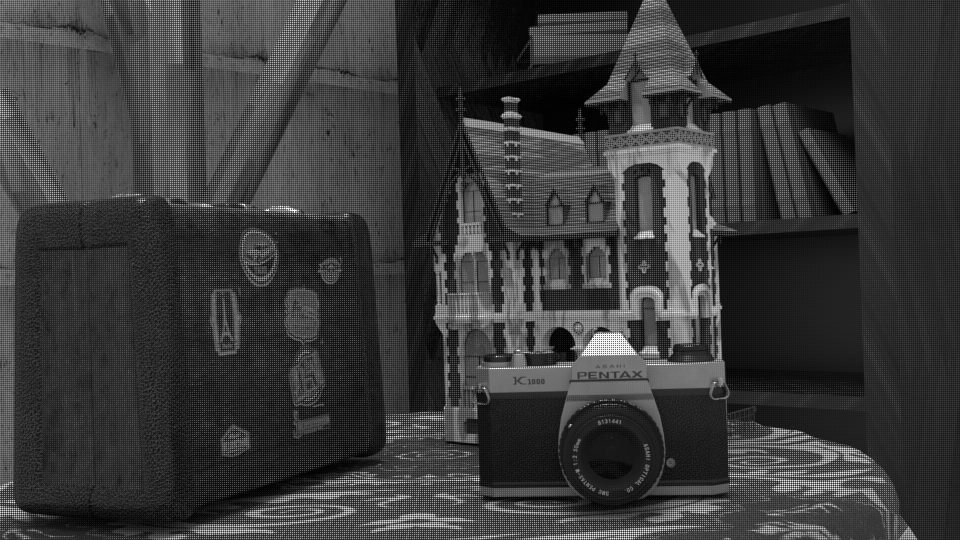
\includegraphics[width=8cm]{bayer_cam2.png}
    \caption{bayer image.}
    \label{fig:result1}
\end{figure}

\begin{figure}[!h]
    \centering
    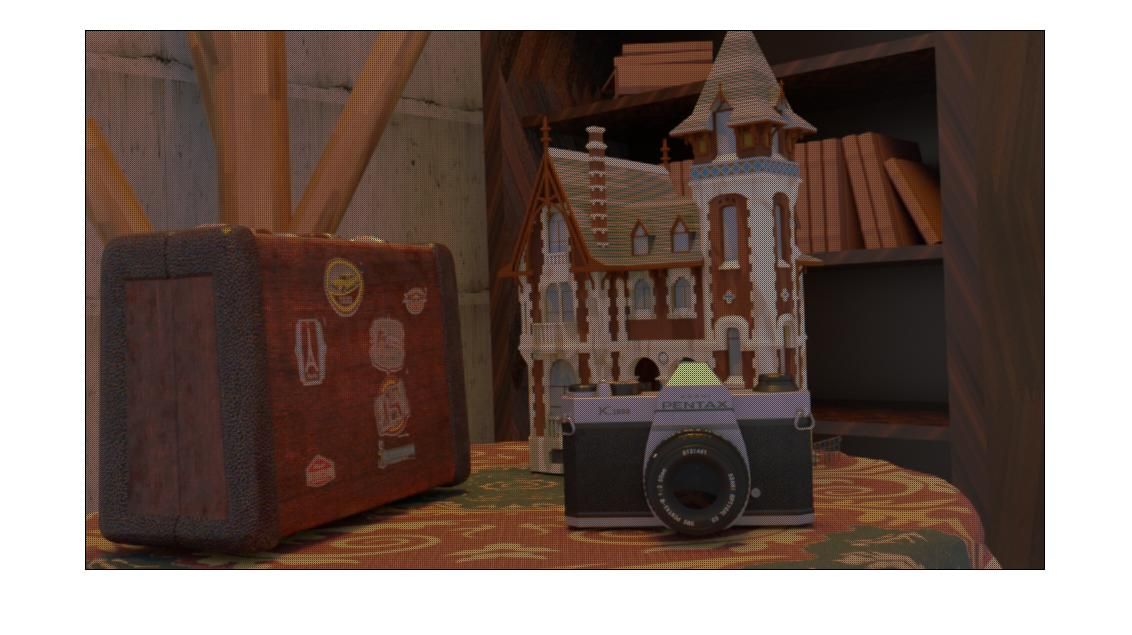
\includegraphics[width=10cm]{1.jpg}
    \caption{bayer to rgb image.}
    \label{fig:result2}
\end{figure}

\newpage
{\large $2.$ calculate\_fundamental\_matrix.m \par}
{\large $3.$ calculate\_rectification\_matrix.m \par}
\begin{figure}[!h]
    \centering
    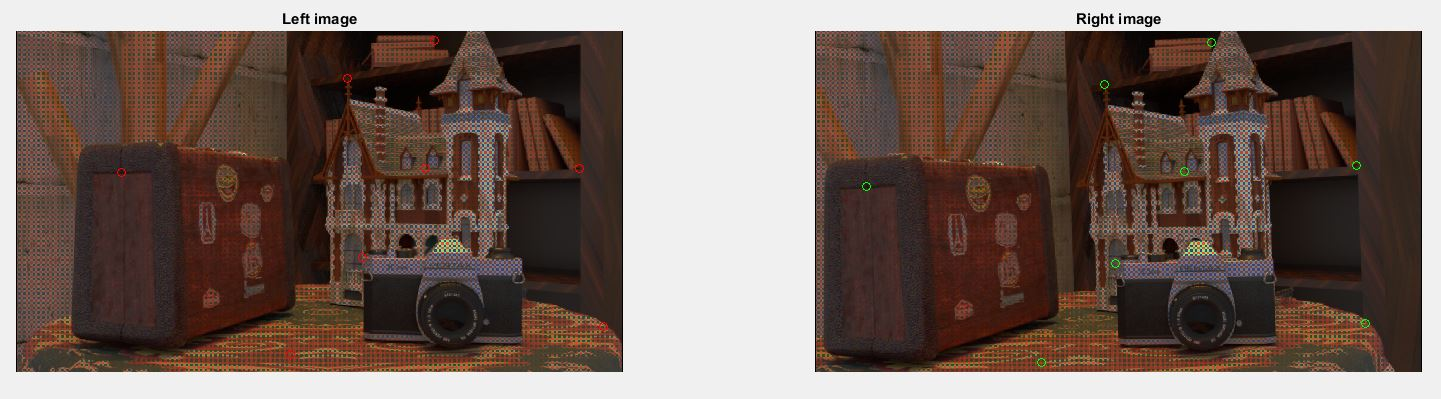
\includegraphics[width=14cm]{22.jpg}
    \caption{visualize matching points on images.}
    \label{fig:result3}
\end{figure}

\begin{figure}[!h]
    \centering
    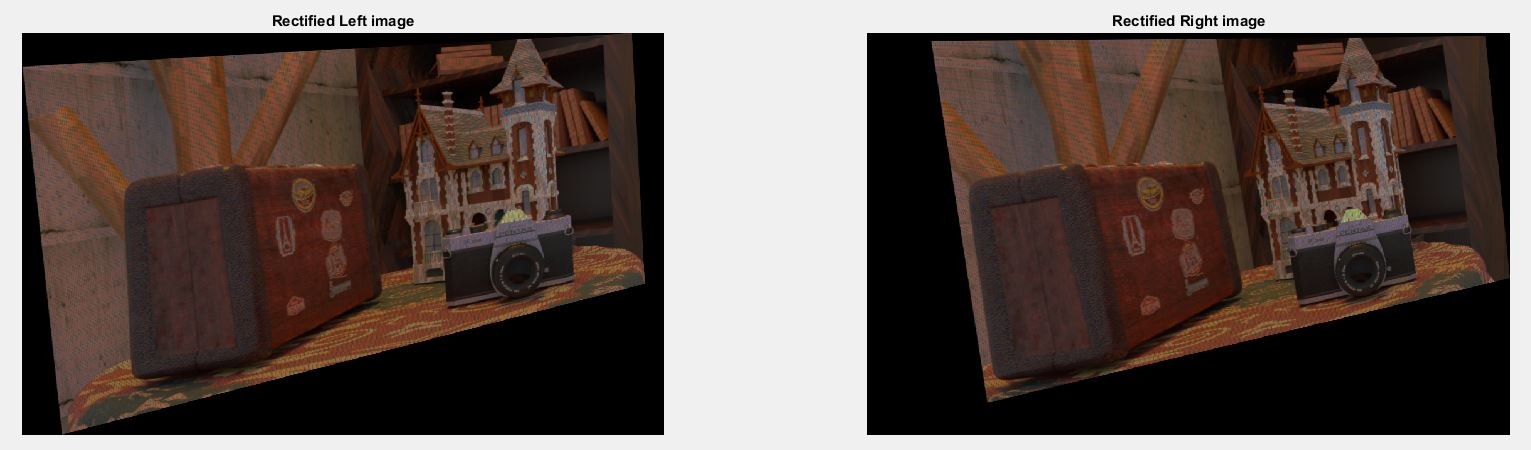
\includegraphics[width=14cm]{33.jpg}
    \caption{visualize rectified images.}
    \label{fig:result4}
\end{figure}

{\large $4.$ calculat\_disparity\_map.m \par}
\begin{figure}[!h]
    \centering
    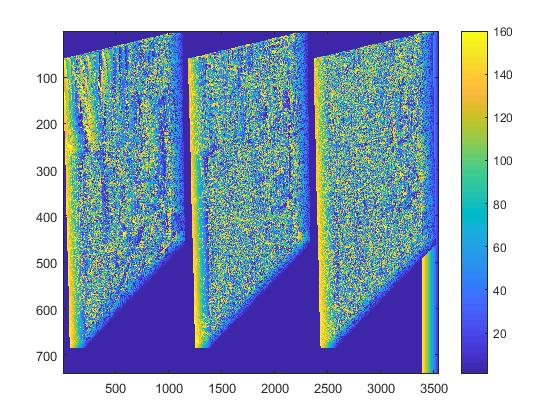
\includegraphics[width=10cm]{5.jpg}
    \caption{visualize rectified images.}
    \label{fig:result5}
\end{figure}

\end{document}